\documentclass[12pt]{article}

\usepackage{cmap}
\usepackage[T2A]{fontenc}
\usepackage[utf8]{inputenc}
\usepackage[russian]{babel}
\usepackage{graphicx}
\usepackage{amsthm,amsmath,amssymb}
\usepackage{listings}
\usepackage{color}
\usepackage[table]{xcolor}
\usepackage{colortbl}
\usepackage{array}
\usepackage{epigraph}
\usepackage{textcomp}

\usepackage[russian,colorlinks=true,urlcolor=red,linkcolor=blue]{hyperref}
\usepackage{enumerate}
\usepackage[shortlabels]{enumitem}
\usepackage{datetime}
\usepackage{fancyhdr}
\usepackage{lastpage}
\usepackage{verbatim}
\usepackage{tikz}
\usetikzlibrary{arrows,patterns,decorations.markings,decorations.pathmorphing,decorations.pathreplacing}
\usetikzlibrary{math,positioning}
\usepackage{pgfplots}

\usepackage{ifthen}
\usepackage{mathtools}
\usepackage{mdframed}
\usepackage[normalem]{ulem}

\graphicspath{ {notes-14-vae} }

\def\SEASON{2024/25}


\sloppy
\voffset=-20mm
\textheight=235mm
\hoffset=-22mm
\textwidth=180mm
\headsep=12pt
\footskip=20pt

\parskip=0em
\parindent=0em

\setlength\epigraphwidth{.8\textwidth}

\newlength{\tmplen}
\newlength{\tmpwidth}
\newlength{\storelen}
\newcounter{listcounter}

% Список с маленькими отступами
\newenvironment{MyList}[1][4pt]{
  \begin{enumerate}[1.]
  \setlength{\parskip}{0pt}
  \setlength{\itemsep}{#1}
}{       
  \end{enumerate}
}
% Вложенный список с маленькими отступами
\newenvironment{InnerMyList}[1][0pt]{
  \vspace*{-0.5em}
  \begin{enumerate}[(a)]
  \setlength{\parskip}{-0pt}
  \setlength{\itemsep}{#1}
}{       
  \end{enumerate}
  \vspace*{-0.5em}
}
% Список с маленькими отступами
\newenvironment{MyItemize}[1][4pt]{
  \begin{itemize}
  \setlength{\parskip}{0pt}
  \setlength{\itemsep}{#1}
}{       
  \end{itemize}
}

% Основные математические символы
\def\TODO{{\color{red}\bf TODO}}
\def\N{\mathbb{N}}       %
\def\R{\mathbb{R}}       %
\def\F2{\mathbb{F}_2}    %
\def\Z{\mathbb{Z}}       %
\def\H{\mathcal{H}}      % семество хеш-функций
\def\E{\mathsf{E}}       % матожидание
\def\INF{\infty}    % +inf
\def\EPS{\varepsilon}    %
\def\EMPTY{\varnothing}  %
\def\PHI{\varphi}        %
\def\SO{\Rightarrow}     % =>
\def\EQ{\Leftrightarrow} % <=>
\def\t{\texttt}          % mono font
\def\c#1{{\rm\sc{#1}}}   % font for classes NP, SAT, etc
\def\O{\mathcal{O}}      %
\def\NO{\t{\#}}          % #
\def\XOR{\text{ {\raisebox{-2pt}{\ensuremath{\Hat{}}}} }}
\def\xor{\t{\^{}}}
\renewcommand{\le}{\leqslant}
\renewcommand{\ge}{\geqslant}
\newcommand{\q}[1]{\langle #1 \rangle}               % <x>
\newcommand\URL[1]{{\footnotesize{\url{#1}}}}        %
\newcommand{\sfrac}[2]{{\scriptstyle\frac{#1}{#2}}}  % Очень маленькая дробь
\newcommand{\mfrac}[2]{{\textstyle\frac{#1}{#2}}}    % Небольшая дробь
\newcommand{\score}[1]{{\bf\color{red}{(#1)}}}
\newcommand{\divby}{\mathop{\raisebox{-2pt}{\vdots}}}

\newcommand{\fix}[1]{{\color{fixcolor}{#1}}} % \underline
\def\bonus{\t{\red{(*)}}}
\def\ifbonus#1{\ifthenelse{\equal{#1}{}}{}{\bonus}}
\def\smallsquare{$\scalebox{0.5}{$\square$}$}
\def\vstick{^\t{\textquotesingle}}
\def\bluebox#1{\fcolorbox{blue}{white}{#1}}

\newlength{\myItemLength}
\setlength{\myItemLength}{0.3em}
\def\ItemSymbol{\smallsquare}
\def\Item{\vspace*{\myItemLength}\ItemSymbol \ \ }

\newcommand{\LET}{%
  % [line width=0.6pt]
  \begin{tikzpicture}%
  \draw(0.8ex,0) -- (0.8ex,1.6ex);%
  \draw(0,1.6ex) -- (0.8ex,1.6ex);%
  \end{tikzpicture}%
  \hspace*{0.1em}%
}

% Отступы
\def\makeparindent{\hspace*{\parindent}\unskip}
\def\up{\vspace*{-0.5em}}%{\vspace*{-\baselineskip}}
\def\down{\vspace*{0.5em}}
\def\LINE{\vspace*{-1em}\noindent \underline{\hbox to 1\textwidth{{ } \hfil{ } \hfil{ } }}}
\def\BOX#1{\mbox{\fbox{\bf{#1}}}}
\def\Pagebreak{\pagebreak\vspace*{-1.5em}}
\def\RIGHT{\hspace*{\fill}} % сдвинуться до упора вправо
\def\NewLine{\hspace*{1em}\\}

% Мелкий заголовок
\newcommand{\THEE}[1]{
  \vspace*{0.5em}
  \noindent{\bf \underline{#1}}%\hspace{0.5em}
  \vspace*{0.2em}
}
% Другой тип мелкого заголовка
\newcommand{\THE}[1]{
  \vspace*{0.5em} $\bullet$
  \noindent{\bf #1}%\hspace{0.5em}
  \vspace*{0.2em}
}

\newenvironment{MyTabbing}{
  \t\bgroup
  \vspace*{-\baselineskip}
  \begin{tabbing}
    aaaa\=aaaa\=aaaa\=aaaa\=aaaa\=aaaa\kill
}{
  \end{tabbing}
  \t\egroup
}

% Код с правильными отступами
\lstnewenvironment{code}{
  \lstset{}
%  \vspace*{-0.2em}
}%
{
%  \vspace*{-0.2em}
}
\lstnewenvironment{codep}{
  \lstset{language=python}
}%
{
}
% Код, содержащий выскоие формулы, вставить не так просто...
\def\codeinput#1{
  \begin{mdframed}[innertopmargin=-2pt,innerbottommargin=-2pt,innerleftmargin=4pt,backgroundcolor=lightgray]
  \lstinputlisting[frame={}]{#1}
  \end{mdframed}
}

% Формулы с правильными отступами
\newenvironment{smallformula}{
 
  \vspace*{-0.8em}
}{
  \vspace*{-1.2em}
  
}
\newenvironment{formula}{
 
  \vspace*{-0.4em}
}{
  \vspace*{-0.6em}
  
}

% Большая квадратная скобка
\makeatletter
\newenvironment{sqcases}{%
  \matrix@check\sqcases\env@sqcases
}{%
  \endarray\right.%
}
\def\env@sqcases{%
  \let\@ifnextchar\new@ifnextchar
  \left\lbrack
  \def\arraystretch{1.2}%
  \array{@{}l@{\quad}l@{}}%
}
\makeatother

% Определяем основные секции: \begin{Lm}, \begin{Thm}, \begin{Def}, \begin{Rem}
\renewcommand{\qedsymbol}{$\blacksquare$}
\theoremstyle{definition} % жирный заголовок, плоский текст
\newtheorem{Thm}{Th}[subsection] % нумерация будет "<номер subsection>.<номер теоремы>"
\newtheorem{Lm}[Thm]{Lm} % Нумерация такая же, как и у теорем
\newtheorem{Ex}[Thm]{Упражнение} % Нумерация такая же, как и у теорем
\newtheorem{Example}[Thm]{Пример} % Нумерация такая же, как и у теорем
\newtheorem{Code}[Thm]{Код} % Нумерация такая же, как и у теорем
\theoremstyle{plain} % жирный заголовок, курсивный текст
\newtheorem{Def}[Thm]{Def} % Нумерация такая же, как и у теорем
\newtheorem{Algo}[Thm]{Алгоритм} % Нумерация такая же, как и у теорем
\theoremstyle{remark} % курсивный заголовок, плоский текст
\newtheorem{Cons}[Thm]{Следствие} % Нумерация такая же, как и у теорем
\newtheorem{Conj}[Thm]{Гипотеза} % Нумерация такая же, как и у теорем
\newtheorem{Prop}[Thm]{Утверждение} % Нумерация такая же, как и у теорем
\newtheorem{Rem}[Thm]{Замечание} % Нумерация такая же, как и у теорем
\newtheorem{Remark}[Thm]{Замечание} % Нумерация такая же, как и у теорем
\newtheorem{Img}[Thm]{Иллюстрация} % Нумерация такая же, как и у теорем

\def\SectionName{Название секции}
\def\AuthorName{Тихонов Даниил}

\newlength{\sectionvskip}
\setlength{\sectionvskip}{0.5em}
\newcommand{\Section}[5][]{
  % Заголовок
  \pagebreak
%  \ifthenelse{\isempty{#1}}{
    \refstepcounter{section}
%  }{}
  \vspace{0.5em}
%  \ifthenelse{\isempty{#1}}{
%    \addtocontents{toc}{\protect\addvspace{-5pt}}%
    \addcontentsline{toc}{section}{\arabic{section}. #2}
%  }{}
  \begin{center}
    {\Large \bf Лекция \NO{#4}: #2} \\ 
    \vspace{\sectionvskip}
    \ifthenelse{\equal{#3}{}}{}{{\large #3}\\}
    % {\large #3} \\
  \end{center}

  \LINE

  % Запомнили название и автора главы
  \gdef\SectionName{#2}
  \gdef\AuthorName{#4}

  % Заголовок страницы
  \lhead{Глубинное обучение 1, \SEASON}
  \chead{}
  \rhead{ФКН ВШЭ}
  \renewcommand{\headrulewidth}{0.4pt}

  \lfoot{Лекция \NO{#4}. #3.}
  \cfoot{\thepage\t{/}\pageref*{LastPage}}
  \rfoot{Лектор: Шипилов Фома}
  \renewcommand{\footrulewidth}{0.4pt}
}

\newcommand{\Subsection}[2][]{
  \refstepcounter{subsection}
  \vspace*{1em}
  \ifthenelse{\equal{#1}{}}
    {\addcontentsline{toc}{subsection}{\arabic{section}.\arabic{subsection}. #2}}
    {\addcontentsline{toc}{subsection}{\arabic{section}.\arabic{subsection}. \bonus\,#2}}
  {\color{blue}\bf\large \arabic{section}.\arabic{subsection}. \ifbonus{#1}\,{#2}} 
  \vspace*{0.5em}
  \makeparindent
}
\newcommand{\Subsubsection}[2][]{
  \refstepcounter{subsubsection}
  \vspace*{1em}
  \ifthenelse{\equal{#1}{}}
    {\addcontentsline{toc}{subsubsection}{\arabic{section}.\arabic{subsection}.\arabic{subsubsection}. #2}}
    {\addcontentsline{toc}{subsubsection}{\arabic{section}.\arabic{subsection}.\arabic{subsubsection}. \bonus\,#2}}
  {\color{blue}\bf\large \arabic{section}.\arabic{subsection}.\arabic{subsubsection}. \ifbonus{#1}\,#2}
  \vspace*{0.5em}
  \makeparindent
}

\newcommand{\Header}{
  \pagestyle{empty}
  \renewcommand{\dateseparator}{--}
  \begin{center}
    {\Large\bf 
     ФКН ВШЭ\\
     %Первый курс, \SEASON\\
    \vspace{0.3em}
    Глубинное обучение 1, \SEASON}\\
    \vspace{0.7em}
    Автор конспекта: Даниил Тихонов \\
    \vspace{0.7em}
    {{\today} в {\currenttime}}
  \end{center}

  \LINE
  \vspace{0em}

  \renewcommand{\baselinestretch}{0.98}\normalsize
  \tableofcontents
  \renewcommand{\baselinestretch}{1.0}\normalsize
  \pagebreak
}

\newcommand{\BeginConspect}{
  \pagestyle{fancy}
  \setcounter{page}{1}
}

\def\Bibliography#1#2#3{\href{#1}{\t{[#2]}}. #3}
\def\Link#1#2#3{\href{#1}{\t{[#2]}}. #3}
\def\ShortLink#1#2{\href{#2}{\t{[#1]}}}

\definecolor{mygray}{rgb}{0.7,0.7,0.7}
\definecolor{ltgray}{rgb}{0.9,0.9,0.9}
\definecolor{fixcolor}{rgb}{0.7,0,0}
\definecolor{red2}{rgb}{0.7,0,0}
\definecolor{dkred}{rgb}{0.4,0,0}
\definecolor{dkblue}{rgb}{0,0,0.6}
\definecolor{dkgreen}{rgb}{0,0.6,0}
\definecolor{brown}{rgb}{0.5,0.5,0}

\newcommand{\green}[1]{{\color{green}{#1}}}
\newcommand{\black}[1]{{\color{black}{#1}}}
\newcommand{\red}[1]{{\color{red}{#1}}}
\newcommand{\dkred}[1]{{\color{dkred}{#1}}}
\newcommand{\blue}[1]{{\color{blue}{#1}}}
\newcommand{\dkgreen}[1]{{\color{dkgreen}{#1}}}


\setlength\parindent{20pt} 

\begin{document}

\Header
\BeginConspect

\Section{Вариационный автокодировщик (VAE)}{27 февраля, 2025}{14}

\Subsection{Manifold Hypothesis}

Прежде чем начинать говорить об автокодировщиках (автоэнкодерах), стоит обосновать законность дальнейших действий, и почему это должно теоретически работать. \\

\fbox{\begin{minipage}{0,95\textwidth}
\textbf{Manifold Hypothesis} 

Гипотеза гласит о том, что б\'oльшая часть присущих реальному миру многомерных данных (картинки, тексты, видео, звук, графы и т.д.) в действительности лежит на низкоразмерном многообразии живущем в многомерном пространстве.
\end{minipage}} \\\\

Другими словами, несмотря на то, что очень часто данные описываются огромным количеством разных признаков (комбинации пикселей на картинке, $n$-грамм в тексте), в реальности только небольшое и хорошо структурированное подмножество комбинаций соответствует настоящим данным, а остальную часть пространства входов составляют нереалистичные объекты. \\

Заметим, что данное знание можно использовать для задачи понижения размерности. Исходя из истинности гипотезы можно построить такое отображение в маломерное пространство признаков, что все свойства объектов в нем сохранятся. 

\Subsection{Понижение размерности}

Пусть имеются многомерные объекты $x \in \R^{D}$, которые мы хотим отобразить в скрытые (\textbf{латентные}) представления $z \in \R^d$, то есть найти

\[
f: \R^D \rightarrow \R^{d}, \quad f(x) = z, \quad d < D \,\, (d \ll D)
\]

Для начала рассмотрим простой случай, когда отображение $f$ линейно. Имея в нашем распоряжении $N$ объектов для обучения, удобно представить задачу в матричном виде: 

\[
X \in \R^{N \times D}, \,\, Z \in \R^{N \times d} \Longrightarrow f(X) = X \Theta = Z, \quad \text{где } \Theta \in \R^{D \times d}
\]

Осталось поставить задачу поиска $\Theta$ так, чтобы латентные представления $Z$ были действительно информативными. Для этого естественно ввести дополнительное ограничение: мы хотим уметь реконструировать исходные объекты $X$ по их скрытым представлениям $Z:$

\[
\hat{X} = Z\Phi, \quad \text{где } \Phi \in \R^{d \times D}
\]

Взяв в качестве лосса обычный MSE, задача обучения принимает вид

\[
\text{MSE}(X, \, \hat{X}) = \Vert X - \hat{X} \Vert_F^2 = \Vert X - Z\Phi \Vert_F^2 = \Vert X - X \Theta \Phi \Vert_F^2 \longrightarrow \min_{\Theta, \Phi}
\]
\[
A = (a_{ij})_{i, j =1}^{n, m} \Longrightarrow \Vert A \Vert_F = \left({\sum_{i, j = 1}^{n, m} |a_{ij}|^2}\right)^{1/2}
\]

\pagebreak

Заметим, что данная задача сводится к малоранговому приближению матрицы:
\[
\hat{X} = X\underbrace{\Theta}_{d \times D} \underbrace{\Phi}_{D \times d} \Longrightarrow rk(\hat{X}) = rk\left(X\Theta \Phi\right) \leq d
\]

В сущности это называется методом главных компонент (PCA) и решается аналитически. 

\Subsection{Autoencoder}

Теперь рассмотрим более сложный случай, где уже нет понятного решения. Если быть конкретнее, разрешим отображению $f$ быть нелинейным, а именно параметризоваться нейросетью. \\

Схема кодирования и декодирования будет иметь следующую bottleneck структуру:

\begin{center}
    \begin{tikzpicture}
        % Границы фигуры
        \draw[thick] (-3,2) -- (-0.5,0.75) -- (0.5,0.75) -- (3,2);
        \draw[thick] (-3,-2) -- (-0.5,-0.75) -- (0.5,-0.75) -- (3,-2);
        \draw[thick] (-3,2) -- (-3,-2);
        \draw[thick] (3,2) -- (3,-2);
        
        % Центральная область (сжатое пространство z)
        \draw[thick] (-0.5,0.75) -- (-0.5,-0.75);
        \draw[thick] (0.5,0.75) -- (0.5,-0.75);
        
        % Подписи
        \node[left] at (-3.25,0) {\Huge $X$};
        \node[right] at (3.25,0) {\Huge $\hat{X}$};
        \node[above] at (0,-0.25) {\Huge $z$};
        \node[below] at (-1.8,0.5) {\Large $f_{\theta}$};
        \node[below] at (1.8,0.5) {\Large $f_{\varphi}$};
        \node[below] at (-1.8,-1.9) {\Large encoder};
        \node[below] at (1.8,-1.9) {\Large decoder};
    \end{tikzpicture}
\end{center}

\fbox{\begin{minipage}{0,95\textwidth}
Тут $f_{\theta}, \, f_{\varphi}$ -- нейросети с параметрами $\theta$ и $\varphi$ соответственно. $f_{\theta}$ называется \textbf{энкодером}, так как кодирует исходные объекты $x$ в латентные представления $z$. $f_{\varphi}$ называется \textbf{декодером}, так как восстанавливает из латентного представления $z$ исходный объект $x$.

\end{minipage}} \\\\

Обозначим за $\mathcal{X}$ распределение наших данных (в реальности конечная выборка). Тогда лосс, на который мы будем учить модель, будет очень похож на MSE:

\[
\mathbb{E}_{x \sim \mathcal{X}}\bigg[\Vert x-\hat{x}\Vert_2^2\bigg] = 
\mathbb{E}_{x \sim \mathcal{X}}\bigg[\Vert x-f_{\varphi}(f_{\theta}(x))\Vert_2^2\bigg]
\longrightarrow \min_{\varphi, \, \theta}
\] \\

На этом этапе логично задаться вопросом. Что будет в случае $d > D$?

\begin{center}
    \begin{tikzpicture}
        % Границы фигуры
        \draw[thick] (-3,0.5) -- (-0.5,2) -- (0.5,2) -- (3,0.5);
        \draw[thick, red] (-3,-0.5) -- (-0.5,-2) -- (0.5,-2) -- (3,-0.5);
        \draw[thick, red] (-3, 0.5) -- (-0.5, -1);
        \draw[thick, red] (3, 0.5) -- (0.5, -1);
        \draw[thick, red] (-0.5, -1) -- (0.5, -1);
        \draw[thick, red] (-3,0.5) -- (-3,-0.5);
        \draw[thick, red] (3,0.5) -- (3,-0.5);
        
        % Центральная область (сжатое пространство z)
        \draw[thick] (-0.5,2) -- (-0.5,-2);
        \draw[thick] (0.5,2) -- (0.5,-2);

        \fill[pattern=north east lines, pattern color=green] (-0.5,2) -- (0.5,2) -- (0.5,-1) -- (-0.5,-1) -- cycle;
        \fill[pattern=north east lines, pattern color=red] (-0.5,-1) -- (0.5,-1) -- (0.5,-2) -- (-0.5,-2) -- cycle;

        
        % Подписи
        \node[left] at (-3.25,0) {\Huge $X$};
        \node[right] at (3.25,0) {\Huge $\hat{X}$};
        \node[above] at (0,-0.25) {\Huge $z$};
        \node[below] at (-1.8,0.8) {\Large $f_{\theta}$};
        \node[below] at (1.8,0.8) {\Large $f_{\varphi}$};
        \node[below] at (-2.7,-1.25) {\Large encoder};
        \node[below] at (2.7,-1.25) {\Large decoder};
        \node[below, green] at (0, 3) {\Large Noise};
        \node[below] at (0, -1) {\Large $\tilde X$};
    \end{tikzpicture} 
\end{center}

    \pagebreak

    Можно было подумать, что модель будет выучивать какие-то новые признаки в латентном представлении, которых не было в исходных объектах. \\
    
    Но на самом деле единственная цель любой нейросети -- минимизация лосса $\Longrightarrow$ в таком сетапе модель скорее всего в каком-то виде скопирует $x$ в латентное представление, а оставшаяся часть будет заполнена шумом, который модель будет полностью игнорировать. \\

    Как все это применять и для чего? Например, автоэнкодеры можно использовать для визуализации многомерных данных: задав латентное представление двумерным или трехмерным, можно отрисовать объекты и глазками попытаться найти какие-то зависимости в данных. \\

    Однако в общем, задача понижения размерности сама по себе является скорее вспомогательной, нежели самодостаточной. Маловероятна ситуация, при которой приходит заказчик и просит решить задачу понижения размерности. 

\Subsection{Denoising Autoencoder}

    Более полезной постановкой, имеющей прямое практическое применение, будет задача расшумления данных. Например, на аудиозаписи голоса в какой-то момент появляется шум сверления у соседей, который хочется научиться убирать. Идея: будем подавать в энкодер зашумленные данные (аудиодорожка), а на выходе из декодера ожидать чистые данные (только голос). \\

    Формально, пусть $\tilde{x}$ -- зашумленный объект, $x$ -- целевой объект без шума, где
    \[
    \tilde{x} = x + \varepsilon, \quad \varepsilon \sim \mathcal{N}(0, \, \sigma^2 I)
    \]
    \[
    \mathbb{E}_{x \sim \mathcal{X}}\bigg[\Vert x-f_{\varphi}(f_{\theta}(\textcolor{red}{\tilde{x}}))\Vert_2^2\bigg]
    \longrightarrow \min_{\varphi, \, \theta}
    \]

    Конкретно в этом примере шум генерируется нормальный, но все как обычно зависит от задачи. В данные, которые мы будем подавать энкодеру на обучении, нужно закладывать какой именно шум мы хотим восстанавливать. \\

    Заметим, что для того, чтобы все это обучить, нам нужны чистые данные. Соответственно, придется один раз потратиться на сбор очень качественных примеров, на которые потом будет накладываться синтетический шум.

    \Subsection{Семплирование}

    До сих пор обсуждались только supervised задачи, но изначально хотелось использовать автоэнкодер в качестве генеративной модели, которая умеет семплировать новые объекты. \\

    Первая идея, которая приходит в голову: давайте оставим только декодер, а генерировать объекты будем следующим образом:
    \[
    z \sim \mathcal{N}(0, \, I) \Longrightarrow x_{gen} = f_{\varphi}(z)
    \]

    \pagebreak

    К сожалению, такая вещь не заведется. Почему? Если мы возьмем $z$, который получился из энкодинга какого-то объекта, то декодер справится с некоторыми поправками восстановить исходный объект. Однако при обучении модели у нас нет никаких гарантий на вид распределения представлений, которые приходят декодеру.

    \begin{center}
        \begin{tabular}{cc}
            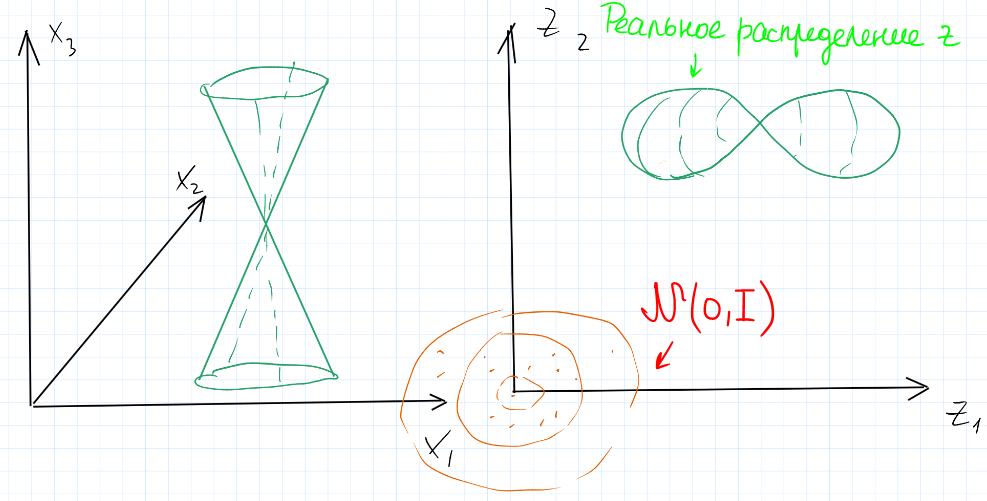
\includegraphics[scale=0.70]{Снимок.PNG}
        \end{tabular}
    \end{center}

    Кажется, что осталась всего одна проблема -- нужно ввести ограничение на то, чтобы распределение на выходах энкодера (входе декодера) было нормальным. Тогда можно будет семплировать привычные для декодера $z$, на которые он учился, и получать новые примеры.

    \Subsection{Variational Autoencoder (VAE)}
    
    Сейчас придется вспомнить модели с латентными переменными (привет EM-алгоритму). Зададим модель на вероятностном языке, а затем поймем, как ее вообще обучать.\\

    Для начала рассмотрим только декодер:

\begin{center}
    \begin{tikzpicture}
        % Границы фигуры
        \draw[thick] (-0.5,0.75) -- (0.5,0.75) -- (3,2);
        \draw[thick] (-0.5,-0.75) -- (0.5,-0.75) -- (3,-2);
        \draw[thick] (3,2) -- (3,-2);
        
        % Центральная область (сжатое пространство z)
        \draw[thick] (-0.5,0.75) -- (-0.5,-0.75);
        \draw[thick] (0.5,0.75) -- (0.5,-0.75);
        
        % Подписи
        \node[right] at (3.25,0) {\Huge $x$};
        \node[above] at (0,-0.25) {\Huge $z$};
        \node[below] at (1.8,0.5) {\Large $f_{\varphi}$};
    \end{tikzpicture}
\end{center}

    \pagebreak

    Запишем совместное распределение $x$ и $z$ при условии параметров $\varphi$ как
    \[
    p(x,  z \, | \, \varphi) = \textcolor{red}{p(x \, | \, z, \varphi)} \, \textcolor{blue}{p(z \, | \, \varphi)} := \textcolor{red}{p(x \, | \, z, \varphi)} \, \textcolor{blue}{p(z)}
    \]

    Первый \textcolor{red}{множитель} как раз отвечает за декодирование: действительно, выход декодера $x$ зависит только от входа $z$ и параметров нейросети декодера $\varphi$. \\

    Второй \textcolor{blue}{множитель} отвечает за распределение латентных переменных $z$, которые мы предполагаем не зависящими от параметров $\varphi$. \\

    Эти распределения мы параметризуем следующим образом:
    \[
    \textcolor{blue}{p(z)} := \mathcal{N}\left(z \, | \, 0, \, I\right)
    \]
    \[
    \textcolor{red}{p(x \, | \, z, \varphi)} := \mathcal{N}\left(x \, | \, \mu_{\varphi}(z), \, \Sigma_{\varphi}(z)\right), \quad \mu_{\varphi}(z) \in \R^{D}, \,\,  \Sigma_{\varphi}(z) \in \R^{D \times D}
    \] 

    Если говорить на языке EM-алгоритма: $x$ являются наблюдаемыми переменными, а $z$ -- латентными. Тогда нашей целью является максимизация следующего правдоподобия: 
    \[
    \log p(x \, | \, \varphi) = \log \int_{\R^d} p(x, z \, | \, \varphi) \, dz \longrightarrow \max_{\varphi}
    \]

    Заметим, что под логарифмом, вообще говоря, интегрируется сложная нейросеть, то есть интеграл не берется. Честно максимизировать правдоподобие не получится, поэтому предлагается облегчить задачу путем вывода нижней вариационной границы (ELBO):
    \[
    \log p(x \, | \, \varphi) = \log p(x \, | \, \varphi) \cdot \textcolor{teal}{1} = \bigg[\text{любое распределение } q(z) \bigg] = \log p(x \, | \, \varphi) \textcolor{teal}{\int_{\R^d} q(z) \, dz} =
    \]
    \[
    = \textcolor{black}{\int_{\R^d} \log p(x \, | \, \varphi) \,q(z) \, dz} = \bigg[p(x \, | \, \varphi) = \frac{p(x, z \, | \, \varphi)}{p(z \, | \, x, \varphi)}\bigg] = \int_{\R^d} q(z) \, \log \frac{p(x, z \, | \, \varphi)}{p(z \, | \, x, \varphi)} \, dz =
    \]
    \[
    = \int_{\R^d} q(z) \, \log \frac{\textcolor{red}{p(x, z \, | \, \varphi)} \, \textcolor{blue}{q(z)}}{\textcolor{blue}{p(z \, | \, x, \varphi)}\, \textcolor{red}{q(z)}} \, dz  = \int_{\R^d} q(z) \, \log \frac{\textcolor{red}{p(x, z \, | \, \varphi)}}{\textcolor{red}{q(z)}} + \int_{\R^d} q(z) \, \log \frac{\textcolor{blue}{q(z)}}{\textcolor{blue}{p(z \, | \, x, \varphi)}} =
    \]
\begin{center}
\fbox{\begin{minipage}{0,50\textwidth}
\[
= \underbrace{\mathcal{L}(q, \,\varphi)}_{\text{ELBO}} + \text{KL}\bigg(q(z) \,\, \big|\big| \,\,p(z \, | \, x, \varphi)\bigg)
\]

\end{minipage}} 
\end{center}

    Таким образом, правдоподобие представилось в виде суммы нижней вариационной оценки и KL-дивергенции между распределением $q$ и апостериорным распределением $p(z \, | \, x, \varphi)$. \\

    Варьируя распределение $q$, можно балансировать между двумя слагаемыми. Если положить распределение на $z$ равным апостериорному при условии данных и параметров, получаем
    \[
    q(z) := p(z \, | \, x, \varphi) \Longrightarrow \text{KL}\bigg(q(z) \,\, \big|\big| \,\,p(z \, | \, x, \varphi)\bigg) = 0 \Longrightarrow {\mathcal{L}(q, \,\varphi)} =  \log p(x \, | \, \varphi)
    \]

    \pagebreak

    Вспомним, что при выводе формулы выше распределение $q$ может быть абсолютно произвольным. В частности, мы можем положить его равным
    \[
    q(z) := q(z \, | \, x, \, \theta), \quad \text{где } \theta \text{ -- параметры энкодера}
    \]

    Это ключевое предположение, которое позволит сделать нашу модель именно автокодировщиком, а не абстрактной моделью с произвольными латентными переменными. То есть $q$ как раз и будет кодировщиком, задающим распределение латентных переменных $z$ при условии входного объекта $x$ и параметров нейросети энкодера $\theta$. \\

    Таким образом, мы получили обе части автоэнкодера:

\begin{center}
    \fbox{\begin{minipage}{0,55\textwidth}
$q(z) := q(z \, | \, x, \, \theta)$ -- энкодер, \quad $p(x \, | \, z, \varphi)$ -- декодер
\end{minipage}} 
\end{center}

    Перепишем ELBO для нового $q$, который и будет лоссом при обучении:
    \[
    \mathcal{L}(q, \, \varphi) = \int_{\R^d} q(z \, | \, x, \theta) \, \log \frac{p(x, z \, | \, \varphi)}{q(z \, | \, x, \theta)} \longrightarrow \max_{\varphi, \, \theta}
    \]

    Осталось определиться с видом распределения, которое задает $q:$
    \[
    q(z \, | \, x, \theta) := \mathcal{N}(z \, | \, \mu_{\theta}(x), \, \Sigma_{\theta}(x))
    \]

    В итоге вся архитектура выглядит следующим образом:

\begin{center}
    \begin{tikzpicture}
        % Границы фигуры
        \draw[thick] (-8.5,2) -- (-8.5,-2);
        \draw[thick] (-0.5,2) -- (-0.5,-2);
        \draw[thick] (-8.5,2) -- (-6.25,0.75);
        \draw[thick] (-8.5,-2) -- (-6.25,-0.75) -- (-6.25, 0.75);
        \draw[thick] (-2.75, 0.75) -- (-0.5, 2);
        \draw[thick] (-2.75, -0.75) -- (-0.5, -2);
        
        % Центральная область (сжатое пространство z)
        \draw[thick] (-3.75,0.75) -- (-3.75,-0.75);
        \draw[thick] (-2.75,0.75) -- (-2.75,-0.75);
        \draw[thick] (-3.75,0.75) -- (-2.75,0.75);
        \draw[thick] (-3.75,-0.75) -- (-2.75,-0.75);
        
        % Подписи
        \node[left] at (-8.75,0) {\Huge $x$};
        \node[right] at (0.5,1.5) {\Large $\mu_{\varphi}(z)$};
        \node[right] at (0.5, -1) {\Large $\Sigma_{\varphi}(z)$};
        \node[above] at (-3.25,-0.25) {\large $z$};
        \node[below] at (-7.3,0.5) {\Large $f_{\theta}$};
        \node[below] at (-1.7,0.5) {\Large $f_{\varphi}$};
        \node[below] at (-5,1.5) {\Large $\mu_{\theta}(x)$};
        \node[below] at (-5,-1) {\Large $\Sigma_{\theta}(x)$};

        % Добавление стрелок к μ и Σ
        \draw[->, thick] (-0.5, 1) to [bend left=30] (0.5, 1.5);
        \draw[->, thick] (-0.5, -1) to [bend right=30] (0.5, -1);

        \draw[->, thick] (-6.25, 0.75) to [bend left=30] (-5.75, 1);
        \draw[->, thick] (-6.25, -0.75) to [bend right=30] (-5.75, -1.25);
    \end{tikzpicture}
\end{center}

    То есть энкодер предсказывает параметры распределения $z$, а декодер -- распределения $x$.\\

    Заметим, что матрицы $\Sigma_{\theta}(x), \, \Sigma_{\varphi}(z)$ имеют размеры $d \times d$ и $D \times D$ соответственно, что очень много уже для каких-нибудь картинок адекватного качества. Поэтому будем предсказывать
    \[
    \Sigma_{\theta}(x) = \text{diag}(\sigma_{\theta_1}^2(x), \dots, \sigma_{\theta_d}^2(x)), \quad \Sigma_{\varphi}(z) = \text{diag}(\sigma_{\varphi_1}^2(z), \dots, \sigma_{\varphi_D}^2(z))
    \]

    Почему хватает диагональной матрицы? Казалось бы, в тех же картинках все соседние пиксели сильно коррелируют. На самом деле нелинейностей внутри энкодера и декодера уже достаточно для моделирования взаимодействий между компонентами, ведь конечное изображение получается из одного латентного вектора $z$, а значит в реальности пиксели будут скоррелированы. На практике можно даже положить $\Sigma_{\varphi}(z) := I$ и все равно будет работать.

    \pagebreak

    Опять запишем полученный лосс:
    \[
    \mathcal{L}(q, \, \varphi) := \mathcal{L}(\theta, \, \varphi) = \int_{\R^d} q(z \, | \, x, \theta) \, \log\frac{p(x, z \, | \, \varphi)}{q(z \, | \, x, \theta)} \, dz = (*)
    \]

    Вспомним, что до этого мы задали совместное распределение как
    \[
    p(x, z \, | \, \varphi) = p(x \, | \, z, \varphi) \, p(z)
    \]

    Подставляя это выражение в лосс, получаем
    \[
    (*) = \int_{\R^d} q(z \, | \, x, \theta) \, \log\frac{p(x \, | \, z, \varphi) \, p(z)}{q(z \, | \, x, \theta)} \, dz = 
    \]
    \[
    = \int_{\R^d} q(z \, | \, x, \theta) \, \log p(x \, | \, z, \varphi) \, dz + 
    \int_{\R^d} q(z \, | \, x, \theta) \, \log\frac{p(z)}{q(z \, | \, x, \theta)} \, dz = 
    \]
\begin{center}
\fbox{\begin{minipage}{0,60\textwidth}
\[
    = \underbrace{\mathbb{E}_{z \sim q(z \, | \, x, \theta)} \bigg[\log p(x \, | \, z, \varphi) \bigg]}_{\text{reconstruction loss (MSE)}} - \underbrace{\text{KL}\bigg(q(z \, | \, x, \theta) \,\, \big|\big| \,\, p(z)\bigg)}_{\text{regularization}}
\]

\end{minipage}} 
\end{center}

    Заметим, что нормальные распределения были заданы не просто так.
    \begin{itemize}
        \item Во-первых, первая компонента лосса в терминах машинного обучения означает, что мы будем просто семплировать батч переменных $z$ и усреднять по нему же. Заметим, что под матожиданием стоит логарифм плотности нормального распределения, а значит это будет тот самый MSE с некоторыми поправками.
        \item Во-вторых, распределения в KL-дивергенции в регуляризационном слагаемом являются нормальными, а значит его можно посчитать аналитически и использовать при обучении.
    \end{itemize}

    По сути, reconstruction loss отвечает за качество восстановленных автоэнкодером объектов, а вторая часть лосса -- регуляризатор, который пытается приблизить латентное распределение $q(z \, | \, x, \theta)$ к априорному распределению $p(z)$, которое мы задали как стандартное нормальное. \\

    В сущности, мы решили ту самую проблему незнания латентного распределения на входе декодера, введя ограничение на его вид и таким образом заставив его быть стандартным нормальным. Теперь для генерации можно семплировать $z \sim \mathcal{N}(0, \, I)$ и прогонять через декодер. \\

    Однако остается еще одна проблема: при обучении нам нужно считать градиент лосса по параметрам $\theta$ и $\varphi$. Со вторым проблем нет, так как $\varphi$ есть только внутри матожидания и градиент спокойно прокидывается. Но как посчитать градиент reconstruction loss по $\theta$, которая есть в параметрах распределения? По сути нужно посчитать градиент операции семплирования.

    \pagebreak
    \Subsection{Reparameterization trick}
    
    Вспомним, следующий факт из теории вероятностей:
    \[
    z \sim \mathcal{N}(z \, | \, \mu_{\theta}(x), \Sigma_{\theta}(x)), \,\, \varepsilon \sim \mathcal{N}(0, \, I) \Longrightarrow 
    z = \mu_{\theta}(x) + \Sigma_{\theta}(x)^{1/2} \varepsilon
    \]

    А значит reconstruction loss можно переписать в виде
    \[
    \mathbb{E}_{z \sim q(z \, | \, x, \theta)} \bigg[\log p(x \, | \, z, \varphi) \bigg] = 
    \mathbb{E}_{\,\varepsilon \sim \mathcal{N}(0, \, I)} \bigg[\log p\left(x \, | \, \mu_{\theta}(x) + \Sigma_{\theta}(x)^{1/2} \varepsilon, \varphi\right) \bigg]
    \]

    Таким образом, мы вытащили параметры $\theta$ из распределения, по которому бралось матожидания, и теперь градиенты можно спокойно считать как и для параметров $\varphi$. \\

    Такая техника называется \textbf{reparameterization trick}. Заметим, что опять же все это удалось провернуть благодаря хорошим свойствам нормального распределения.

    \Subsection{Вывод формулы итогового лосса}

    Посчитаем reconstruction loss для одного $z$:
    \[
    \log p(x \, | \, z, \varphi) = \log \left(\frac{1}{(2\pi)^{D / 2} |\Sigma|^{1/2}} \, \exp\left\{-\frac{1}{2}(x-\mu)^T\Sigma^{-1}(x-\mu)\right\}\right) =
    \]
    \[
    = -\frac{D}{2}\, \log 2\pi - \frac{1}{2} \, \log |\Sigma| - \frac{1}{2} \, (x - \mu)^T\Sigma^{-1}(x-\mu) =\text{const}(\mu, \,\Sigma) - \frac{1}{2}\sum_{i=1}^D \sigma_i^2 - \frac{1}{2} \sum_{i=1}^D \frac{(x_i - \mu_i)^2}{\sigma_i^2}
    \]
    
    Если для декодера взять $\Sigma_{\varphi}(z) = I$, получим
    \[
     \log p(x \, | \, z, \varphi) \propto -\frac{1}{2} \sum_{i=1}^D (x_i - \mu_i)^2 \Longrightarrow -\frac{1}{2}\text{MSE},
    \]
    \[
    \text{где } x_i \text{ -- исходный объект, а } \mu_i \text{ -- выход декодера} 
    \]

    Теперь распишем слагаемое, отвечающее за регуляризацию. Для этого вспомним, что
    \[
    \xi_1 \sim \mathcal{N}(\xi_1 \, | \, \mu_1, \, \Sigma_1), \,\, \xi_2 \sim \mathcal{N}(\xi_2 \, | \, \mu_1, \, \Sigma_2)
    \]
    \[
    \Longrightarrow \text{KL}\big(\xi_1 \,\, \big|\big| \,\,\xi_2 \big) = \frac{1}{2} \bigg[tr\left(\Sigma_2^{-1}\Sigma_1\right) -d + (\mu_2 - \mu_1)\Sigma_2^{-1}(\mu_2 - \mu_1)+ \ln \frac{|\Sigma_2|}{|\Sigma_1|}\bigg]
    \]

    Таким образом, полагая $\Sigma_{\theta} = \text{diag}(\sigma_1^2, \dots, \sigma_d^2)$:
    \[
    \text{KL}\bigg(q(z \, | \, x, \theta) \,\, \big|\big| \,\, p(z)\bigg) = \frac{1}{2} \bigg[tr\left(\Sigma_{\theta}\right) - d + ||\mu_{\theta}||_2^2- \log \Sigma_{\theta}\bigg] = -\frac{d}{2} - \frac{1}{2} \sum_{i=1}^d \left(\sigma_i^2 + \mu_i^2 - \log \sigma_i^2\right)
    \]
\begin{center}
\fbox{\begin{minipage}{0,95\textwidth}
Для того, чтобы всегда получать неотрицательные значения $\sigma_i^2$, будем предсказывать $\log \sigma_i^2$, а затем экспоненциировать это значение для получения дисперсии.
\end{minipage}} 
\end{center}

\pagebreak

    \Subsection{Заключение}

    Сравнивая с GANами, вариационный автоэнкодер решает проблему mode collapse, от которой сильно страдают первые. Семплы получаются более разнообразные, покрывается все распределение данных. \\

    С другой стороны, картинки в GANах получаются очень хорошего качества, максимально реалистичные. Вариационный автоэнкодер в свою очередь генерирует более размытые изображения, которые легко отличить от реальных. Это происходит из-за приближения пикселей нормальным распределением, что не соответствует действительности. \\

    Вывод: для генерации картинок, где важно качество, и mode collapse не так критичен, стоит использовать GANы. Если же для задачи очень важно покрывать все разнообразие распределения, как в биоинформатике или физике, разумнее будет выбрать VAE.
    
     


    

    





\end{document}
